% 微分的几何意义
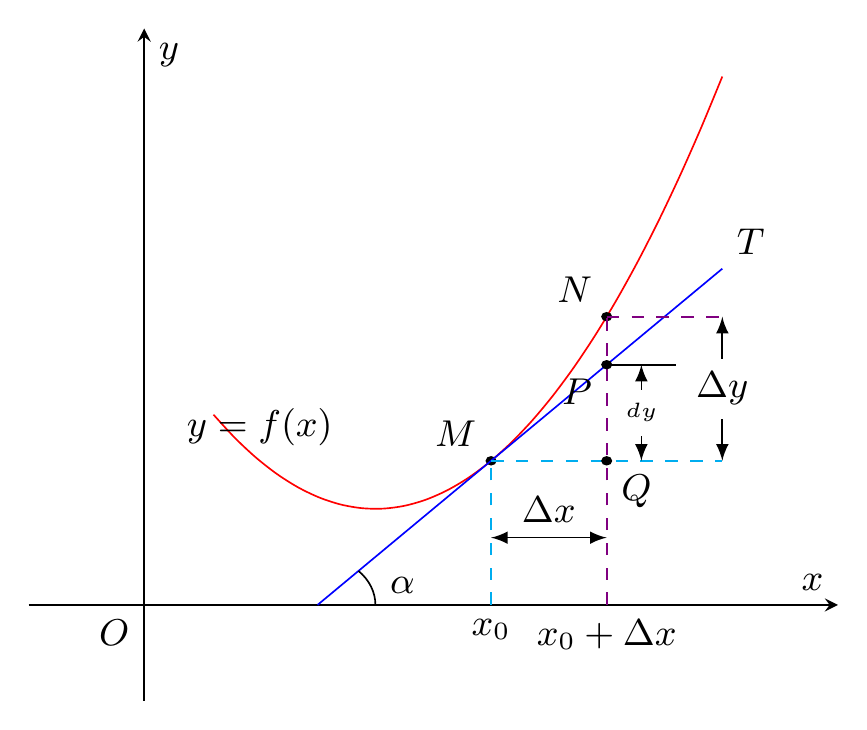
\begin{tikzpicture}[scale = 1.5]
  \begin{axis}[clip=false,xmin=-0.5, xmax=3,ymin=-0.5,ymax=3, grid=none,
    xtick=\empty, ytick=\empty, font=\small, axis lines=middle,
    smooth, xlabel={$x$}, ylabel={$y$}]

    % 曲线
    \addplot[draw=red,domain=0.3:2.5] {(x - 1)^2 + 0.5};
    \node [above] at (0.5,0.75) {$y = f(x)$};
    \draw[fill] (1.5,0.75) circle [radius=0.02];
    \draw[fill] (2,1.5) circle [radius=0.02];
    % 切线
    \addplot[draw=blue,domain=0.75:2.5] {x - 0.75};
    \node [above right] at (2.5,1.75) {$T$};

    % 辅助线和点
    \draw [dashed, draw=cyan] (1.5, 0) -- (1.5, 0.75);
    \draw [dashed, draw=cyan] (1.5, 0.75) -- (2.5, 0.75);
    \node [above left] at (1.5,0.75) {$M$};
    \node [below] at (1.5,0) {$x_0$};

    % \Delta x
    \draw [latex-latex] (1.5, 0.35) -- (2, 0.35);
    \node [above] at (1.75,0.35) {$\Delta x$};

    % \Delta y
    \draw [latex-latex] (2.5, 0.75) -- (2.5, 1.5);
    \node [fill=white] at (2.5,1.125) {$\Delta y$};

    % dy
    \draw (2, 1.25) -- (2.3, 1.25);
    \draw [latex-latex] (2.15, 0.75) -- (2.15, 1.25);
    \node [fill=white, font=\tiny] at (2.15,1) {$dy$};

    \draw [dashed, draw=violet] (2, 0) -- (2, 1.5);
    \draw [dashed, draw=violet] (2, 1.5) -- (2.5, 1.5);
    \node [above left] at (2,1.5) {$N$};
    \node [below] at (2,0) {$x_0 + \Delta x$};

    \draw[fill] (2,1.25) circle [radius=0.02];
    \node [below left] at (2,1.25) {$P$};

    \draw[fill] (2,0.75) circle [radius=0.02];
    \node [below right] at (2,0.75) {$Q$};

    % 倾角
    \draw (1,0) arc (0:45:0.25);
    \node [right] at (1,0.1) {$\alpha$};

    % 原点
    \node [below left] at (0,0) {$O$};
  \end{axis}
\end{tikzpicture}
